\documentclass[11pt,openany]{book}
% #1-Asignatura
% #2-Curso
% #3-Nombre
% #4-Link
% #5-Foto

\newcommand{\portada}[5]{
    \begin{titlepage}
        \begin{center}
            \vspace*{0.5cm}
            
            % Titulo con #1 lo mas grande posible
            {\Huge \textbf{#1}}

            
            \vspace{0.5cm}
            \LARGE
            Curso #2 
            
            \vspace{1cm}
            
            \Huge{\textbf{Grupo Viterbi}}

            \vspace{1cm}
            
\includegraphics[width=0.6\textwidth]{assets/Img/UGR-Logo.png}
            
            \vspace{0.5cm}

            \huge
            PRÁCTICA 5- PROGRAMACIÓN DINÁMICA
            
            \Large
            \vspace{1cm}
            \textbf{Integrantes:}  \\ 
             % Array con los nombres de los integrantes y el correo
             \begin{center}
                \begin{tabular}{c c }
                    \textbf{Miguel Ángel De la Vega Rodríguez} & miguevrod@correo.ugr.es \\
                    \textbf{Alberto De la Vera Sánchez} & joaquinrojo724@correo.ugr.es \\
                    \textbf{Joaquín Avilés De la Fuente} & adelaveras01@correo.ugr.es \\
                    \textbf{Manuel Gomez Rubio} & e.manuelgmez@go.ugr.es \\
                    \textbf{Pablo Linari Perez} & e.pablolinari@go.ugr.es
                \end{tabular}
             \end{center}
            \vspace{0.8cm}
            
            
            \large
             \vspace{1cm}
            Facultad de Ciencias UGR\\
            Escuela Técnica Ingeniería Informática UGR\\
            Granada\\
            #2 
            
        \end{center}
    \end{titlepage}
}



\usepackage{assets/formulas}
\usepackage[mathscr]{euscript}
\usepackage{bm}
\usepackage{float}
\hbadness=10000 % Suppress Underfull \hbox warnings

%========================================|Indice|===============================================%

\begin{document}
\portada{Algorítmica}{2023-2024}{Miguel Ángel De la Vega Rodríguez}{https://github.com/Miguevrgo/}{github.png}
\tableofcontents % Índice
\newpage %Salto de pagina tras el Indice


%======================================|Documento|==============================================%
\chapter{Autores}
\begin{itemize}
      \item \textbf{Miguel Ángel De la Vega Rodríguez:} 20\%
            \begin{itemize}
                  \item Algoritmos Greedy del Viajante
                  \item Redacción memoria sección Viajante
            \end{itemize}
      \item \textbf{Joaquín Avilés De la Fuente:} 20\%
            \begin{itemize}
                  \item Programación Branch and Bound
                  \item Programación creación de casos (puntos y matrices de adyacencia)
                  \item Programación de funciones de cota para Branch and Bound
            \end{itemize}
      \item \textbf{Alberto De la Vera Sánchez: } 20\%
            \begin{itemize}
                  \item Programación hijo predilecto
                  \item Redacción hijo predilecto
                  \item Conclusión
            \end{itemize}
      \item \textbf{Manuel Gomez Rubio} 20\%
            \begin{itemize}
                \item Programacion Backtracking
                \item Redacción Backtracking
            \end{itemize}
      \item \textbf{Pablo Linari Pérez:} 20\%
            \begin{itemize}
                  \item Programacion Backtracking
                  \item Redacción Objetivos
                  \item Redacción Backtracking
            \end{itemize}
\end{itemize}

\chapter{Equipo de trabajo}

\begin{itemize}
      \item \textbf{Miguel Ángel De la Vega Rodríguez:} (Ordenador donde se ha realizado el computo)
            \begin{itemize}
                  \item AMD Ryzen 7 2700X 8-Core
                  \item 16 GB RAM DDR4 3200 MHz
                  \item NVIDIA GeForce GTX 1660 Ti
                  \item 1 TB SSD NvMe
                  \item Debian 12 Bookworm
                  \item Compilador GCC 12.2.0
            \end{itemize}
\end{itemize}

\chapter{Objetivos}
    El objetivo de esta práctica es resolver el problema del viajante de comercio el cual viene descrito por el siguiente enunciado :\
    Tenemos un conjunto de n ciudades (puntos en un plano), cada una definida por las coordenadas en el mapa $(x_i , y_i )$, con $i = 1, . . . , n$. La distancia entre dos ciudades viene dada por la
    distancia euclídea entre sus coordenadas.
    El problema de viajante de comercio consiste en encontrar el orden en el que un viajante,
    partiendo de la ciudad de origen (por ejemplo $(x_1 , y_1 )$) pase por todas y cada una de las ciudades
    una única vez, para volver a la ciudad de partida, formando un ciclo. \ 

    Para ello usaremos dos diseños distintos de  algoritmos dedicados a la exploraciónde grafos , backtracking y brannch and bound 
    con el objetivo de ver las diferencias entre la eficiencia de estos dos algoritmos. Además se probarán distintas funciones de cotsa 
    para estudiar que influencia tienen en cada caso las distintas funciones.Por último se realizará un estudio tanto teórico como 
    empírico de la eficiencia de los algoritmos implementados.
\chapter{Backtracking}   
\section{Diseño}   
En esta sección analizaremos el algorimo de exploración de grafos llamado Backtracking, que consiste en recorrer todos los caminos en profundidad obteniendo todas
las posibles soluciones al problema. \\
Para seleccionar la solución más óptima del problema debemos ir comparando con la anterior posible solución  cada vez que obtenemos una nueva solución al problema, quedándonos con la que más nos
convenga, en este caso, la que nos de un camino de menor disatancia.
\\ \\
Hay varias formas de hacerlo:
\begin{itemize}
      \item La primera forma consiste en hacerlo mediante fuerza bruta, es decir, usar la definición al uso de Backtracking recorriendo todos los caminos sin preocuparnos
      si estos nos permiten alcanzar una solución mejor que la obtenida anteriormente.
      \item La otra forma es implementar una función de cota, esto nos permite decidir si seguimos explorando el camino seleccionado porque nos puede dar un resultado mejor
      o si es mejor abandonarlo, ya que no se obtendrá una mejora.
      Esta forma de realizarlo será, como es lógico, más eficiente.
\end{itemize}

Para la implementación del algoritmo, optamos por la segunda forma, usando diferentes funciones de cota que nos permitan aproximar si el camino seleccionado es bueno.A continuación
veremos como se ha elegido cada cota .
\subsection{Cota global}

\begin{lstlisting}
    vector<int> nearest_neighborTSP(const vector<vector<double>>& distancias, int inicial) {
    int num_puntos = distancias.size();
    vector<int> camino;
    vector<bool> visitados(num_puntos, false);
    camino.reserve(num_puntos);
    camino.push_back(inicial);
    visitados[inicial] = true;

    for (int i = 0; i < num_puntos - 1; ++i) {
        int actual = camino.back();
        int siguiente = -1;
        double min_distancia = numeric_limits<double>::max();

        for (int j = 0; j < num_puntos; ++j) {
            if (!visitados[j] && distancias[actual][j] < min_distancia) {
                min_distancia = distancias[actual][j];
                siguiente = j;
            }
        }

        camino.push_back(siguiente);
        visitados[siguiente] = true;
    }

    camino.push_back(inicial);
    return camino;
}
\end{lstlisting} 
Esta funcion de la practica anterior la usaremos par obtener una cota global, ya que nos proporciona una solución al problema del viajante, aunque no sea la mejor, nos servirá para comparar
Si la decision que toma nuestro algoritmo es mejor que la que nos proporciona esta función. 

\subsection{Cota local}
\textbf{Primera función de cota:} \\
    La primera función de cota que hemos implementado consiste en calcular el mínimo valor de los arcos del grafo que no han sido 
    usados todavía , se multiplican por el numero de nodos restantes y se suman al coste actual.
    \begin{lstlisting}
        double cota1(const vector<vector<double>> &graph, const vector<int> &solucion,double c_actual, double arco_menorpeso) {
            return arco_menorpeso * (graph.size() - solucion.size() + 1) + c_actual;
        }

    \end{lstlisting}
\textbf{Segunda función de cota:} \\
    La segunda función de cota que hemos implementado consiste en calcular el mínimo valor de salir de todos los nodos del grafo que no 
    han sido visitados y sumarle la distancia del recorrido actual.
    En el siguiente codigose recorre la matriz de adyacencia y se selecciona el menor valor de los arcos de los nodos que no han sido visitados 
    y se suman al coste actual.
    \begin{listing}
        double cota2(const vector<vector<double>> &graph, const vector<int> &solucion,=double c_actual) {
            double cota = 0;
            vector<double> v;
            double min = numeric_limits<double>::max();
            for (int i = 1; i < graph.size(); ++i) {
                if ((find(solucion.begin(), solucion.end(), i) == solucion.end())) {
                    v = graph[i];
                    sort(v.begin(), v.end());
                    cota += v[1];
                }
            }
            return cota + c_actual;
        }
    \end{listing}
    \textbf{Tercera función de cota:} \\
    La tercera función de cota que hemos implementado consiste en calcular el mínimo valor de salir y entrar  de todos los nodos del grafo que no 
    han sido visitados ,hacer la media  y sumarle la distancia del recorrido actual.
    El siguiente codigo busca en una matriz de adyacencia los valores de los arcos de los nodos que no han sido todavia visitados , se 
    seleccionan todos ellos y se ordenande menor a mayor para seleccionar los dos menores y hacer la media de estos.
    \begin{listing}
        double cota3(const vector<vector<double>> &graph, const vector<int> &solucion,double c_actual) {
            double cota = 0;
            vector<double> v;
            double min = numeric_limits<double>::max();
            for (int i = 1; i < graph.size(); ++i) {
                if ((find(solucion.begin(), solucion.end(), i) == solucion.end())) {
                    v = graph[i];
                    sort(v.begin(), v.end());
                    cota += (v[1] + v[2]) / 2;
                }
            }
            return cota + c_actual;
        }
    \end{listing}
\subsection{Algoritmo Backtracking}
A continuación se muestra el algoritmo de Backtracking implementado:

\begin{lstlisting}
/**
 * @brief Funcion para resolver el tsp con backtracking .
 * @param solucion vector de ciudades , la posicion de la ciudad indica el orden
 * en el que es visitada
 * @param graph graph de adyacencia
 * @param c_mejor mejor coste encontrado
 * @param s_mejor mejor solucion encontrada
 * @param c_actual coste actual
 * @param arco_menorpeso arco de menor peso del grafo (para no tener que calcularlo siempre)
 *@param cota cota a utilizar
 */
 void tsp_backtracking(vector<int> &solucion,const vector<vector<double>> &graph, double &c_mejor,vector<int> &s_mejor, double c_actual, int arco_menorpeso,int cota = 0) {
  c_actual += solucion.size() <= 1? 0: graph[solucion.back()][solucion[solucion.size() - 2]];
  if (solucion.size() == graph.size()) {
    c_actual += graph[solucion.back()][solucion[0]];
    if (c_actual < c_mejor) {
      c_mejor = c_actual;
      s_mejor = solucion;
    }
  } else {
    for (int i = 1; i < graph.size(); i++) {
      if (find(solucion.begin(), solucion.end(), i) == solucion.end()) {
        double acotacion;
        if (cota == 1) {
            acotacion = cota1(graph, solucion, c_actual, arco_menorpeso);
        } else if (cota == 2) {
            acotacion = cota2(graph, solucion, c_actual);
        } else if (cota == 3) {
            acotacion = cota3(graph, solucion, c_actual);
        } else {
            acotacion = 0;
        }
        if (acotacion <= c_mejor) {
            solucion.emplace_back(i);
            tsp_backtracking(solucion, graph, c_mejor, s_mejor, c_actual,arco_menorpeso, cota);
            solucion.pop_back();
          }
      }
    }
  }
}

  
                
    \end{lstlisting}

    El algoritmo recive como parametros una matriz de adyacencia , un vector de enteros que representa la solución actual, un vector de enteros que representa la mejor solución encontrada, un double que representa el mejor coste encontrado, un double que representa el coste actual, un entero que representa el arco de menor peso del grafo y un entero que representa la cota a utilizar.
    El vector de enteros solucion contiene el punto inicial sobre el que se aplica el algoritmo , si el vector solución
    
\section{Justificación}
Para la justificación del Backtracking necesitamos comprobar, en nuestro caso por reducción al absurdo en el paso
de inducción, que la solución obtenida es la mejor posible:
\begin{enumerate}
    \item Llamaremos N al conjunto de todos los nodos 
    \item Llamaremos $C_l$ a la cota local
    \item Llamaremos C a la cota global
    \item Una solución será la óptima cuando se hayan explorado todos los caminos teniendo en cuenta la cota local y global de ese momento
\end{enumerate}
En la inducción sobre N, el caso base es evidente, ya que si hay un único nodo, este será la solución al problema y la distancia recorrida será de 0. Ocurre de igual forma

\section{Eficiencia teórica y empírica}
\subsection{Eficiencia teórica}


\chapter{Branch and bound}
Al igual que en el apartado anterior resolveremos el problema del viajante, solo que en vez de solucionar el problema mediante el bakctraking 
lo resolveremos mediante Branch and bound. A continuación se mostrarán las funciones de cota al igual que el algoritmo principal que hemos usado:

\section{Diseño}
\subsection{Cota global}
Para selecionar la cota global usaremos la función de nearest neighbor de la práctica anterior la cual 
nos proporciona una cota principal con la que poder comparar las distintas soluciones que vaya obteniendo nuestro algoritmo.

\begin{lstlisting}
vector<int> nearest_neighborTSP(const vector<vector<double>>& distancias, int inicial) {
    int num_puntos = distancias.size();
    vector<int> camino;
    vector<bool> visitados(num_puntos, false);
    camino.reserve(num_puntos);
    camino.push_back(inicial);
    visitados[inicial] = true;

    for (int i = 0; i < num_puntos - 1; ++i) {
      int actual = camino.back();
      int siguiente = -1;
      double min_distancia = numeric_limits<double>::max();

      for (int j = 0; j < num_puntos; ++j) {
          if (!visitados[j] && distancias[actual][j] < min_distancia) {
              min_distancia = distancias[actual][j];
              siguiente = j;
          }
      }

      camino.push_back(siguiente);
      visitados[siguiente] = true;
    }

    camino.push_back(inicial);
    return camino;
}

\end{lstlisting} 
\\ 

      
\end{lstlisting}
\subsection{Cota local}

Además de esta cota global, hemos implementado dos funciones de cota local distintas:
\\ 
\begin{lstlisting}
double cota_inferior_1(const std::vector<std::vector<double>>& matriz, const std::vector<int>& indices_a_ignorar = {}) {
    double suma_minimos = 0.0;

    for (int i = 0; i < matriz.size(); ++i) {
        
        if (std::find(indices_a_ignorar.begin(), indices_a_ignorar.end(), i) != indices_a_ignorar.end()) {
            continue;
        }

        double minimo_fila = std::numeric_limits<double>::max();
        for (int j = 0; j < matriz[i].size(); ++j) {
            
            if (std::find(indices_a_ignorar.begin(), indices_a_ignorar.end(), j) != indices_a_ignorar.end()) {
                continue;
            }
            if (matriz[i][j] > 0 && matriz[i][j] < minimo_fila) {
                minimo_fila = matriz[i][j];
            }
        }

        if (minimo_fila < std::numeric_limits<double>::max()) {
            suma_minimos += minimo_fila;
        }
    }

    return suma_minimos;
}    

double cota_inferior_2(const std::vector<std::vector<double>>& matriz, const std::vector<int>& indices_a_ignorar = {}) {
    double min_global = std::numeric_limits<double>::max();
    int filas_contadas = 0;

    for (int i = 0; i < matriz.size(); ++i) {
        
        if (std::find(indices_a_ignorar.begin(), indices_a_ignorar.end(), i) != indices_a_ignorar.end()) {
            continue;
        }

        double minimo_fila = std::numeric_limits<double>::max();
        for (int j = 0; j < matriz[i].size(); ++j) {
            
            if (std::find(indices_a_ignorar.begin(), indices_a_ignorar.end(), j) != indices_a_ignorar.end()) {
                continue;
            }
            if (matriz[i][j] > 0 && matriz[i][j] < minimo_fila) {
                minimo_fila = matriz[i][j];
            }
        }

        if (minimo_fila < std::numeric_limits<double>::max()) {
            if (minimo_fila < min_global) {
                min_global = minimo_fila;
            }
            ++filas_contadas;
        }
    }

    return  (min_global * filas_contadas);
}
            
\end{lstlisting}
La primera función de cota local consiste en calcular el mínimo de una matriz de distancias, excluyendo obviamente los valores
de 0, pasandose como parámetros los índices a ignorar.Destacar que además de obviar dichas filas se obviarán sus respectivas 
columnas indicadas en el vector de enteros, ya que el objetivo es eliminar las conexiones de ciertos nodos, por lo que 
eliminamos sus filas y columnas respectivas.
\\ \\
Por otro lado, la segunda función de cota, tiene un funcionamiento 
distinto. Consiste principalmente en encontrar la mínima distancia de una matriz de adyacencia y depués multiplicar dicho valor por
las filas restantes, suponiendo que ese camino será el mínimo para todos, de ahí que se multiplique por el número de nodos restantes.
Ignorando, igual que con la cota anterior, los 0 y las filas y las columnas que se pasan como parámetros a ignorar. Función para calcular 
cota inferior calculando el mínimo de una matriz de distancias, excluyendo el 0 y las filas. Es claro que este segundo método nos proporciona 
una cota más restrictiva por lo que nos interesa más.
\\ \\
Más adelante en el apartado de eficiencia seguiremos comparando dichas cotas.

\subsection{Algoritmo Branch and Bound}
Primero de todo, el struct con el que trabajaremos para almacenar la información sobre la cota mínima, el camino y la distancia recorrida será:

\begin{lstlisting}
      struct Nodo {
            vector<int> path;
            double distancia_recorrida; 
            double cota_inferior; 
        
            Nodo(vector<int>& inicial, double dist_rec, double cota_inf) {
                path = inicial;
                distancia_recorrida = dist_rec;
                cota_inferior = cota_inf;
            }
      };
\end{lstlisting}

Ahora, el algoritmo Brach and Bound que hemos implementado ha sido:

\begin{lstlisting}
vector<int> branch_and_bound_greedy(vector<int>& points, vector< vector<double>> &distancias, int inicial){
    priority_queue<Nodo, vector<Nodo>, Comparador> no_visitados;
    vector<int> mejor_camino = {inicial};
    Nodo actual( mejor_camino, 0, cota_inferior(distancias));
    no_visitados.push(actual);

    double costo_minimo = calcularDistanciaTotal(distancias, nearest_neighborTSP(distancias, inicial));
    mejor_camino.clear();

    while (!no_visitados.empty()) {
        actual = no_visitados.top();
        no_visitados.pop();

        if (actual.path.size() == points.size()-1) {
            vector<int> faltantes= numeros_faltantes(actual.path, points.size()-1);
            actual.distancia_recorrida += distancias[actual.path.back()][faltantes[0]];
            actual.distancia_recorrida += distancias[faltantes[0]][inicial];
            actual.path.push_back(faltantes[0]);
            actual.path.push_back(inicial);
            if (actual.distancia_recorrida <= costo_minimo) {
                costo_minimo = actual.distancia_recorrida;
                mejor_camino = actual.path;
            }
        } 
        else { 
            if (actual.cota_inferior <= costo_minimo ){
                vector<int> faltantes = numeros_faltantes(actual.path, points.size()-1);
                for (int i = 0; i < faltantes.size(); ++i) {
                    Nodo nuevo= actual;
                    nuevo.path.push_back(faltantes[i]);
                    nuevo.distancia_recorrida += distancias[actual.path.back()][faltantes[i]];
                    nuevo.cota_inferior = nuevo.distancia_recorrida + cota_inferior(distancias, nuevo.path);
                    no_visitados.push(nuevo);
                }
            }
        }
    }

    return mejor_camino;

}
\end{lstlisting}
El funcionamiento de este método se basa en empezar creando un nodo con el punto inicial y agregarlo a la cola de prioridad (cuyo comparador
consiste en comparar la distancia recorrida por un nodo a y un nodo b y ver qué distancia es menor). Mientras la cola no esté vacía; primero,
se extrae el nodo con menor costo actual (a partir de la cota inferior y haciendo uso del comparador definido anteriormente); si el camino actual 
tiene todos los puntos menos unos, sabemos de forma determinada cual queda mediante la función faltantes de antes(dicha función encuentra los números
faltantes desde 0 hasta n en un vector de enteros), por lo que se calcula la distancia a dicho punto y al inicial y se agrega a la solución si es 
mejor que la actual; si no, se generan los nodos hijos con los puntos faltantes y se agregan a la cola de prioridad.
\\ \\
A continuación se mostrará la notación mostrada en teoría, aunque sigamos un esquema similar, hay ciertos ámbitos que pueden ser suprimidos.
\\\\
\textbf{Notación:}
\begin{itemize}
      \item \textbf{Solución parcial:} Vector path del Nodo actual.
      \item \textbf{Función poda:} Momento en que la cota inferior supera al costo minimo,siendo este la cota global.
      \item \textbf{Restricciones explícitas:}Que el siguiete nodo a seleccionar este dentro de los nodos faltantes
      \item \textbf{Restricciones implícitas:}Que el camino del nodo actual sea menor que el costo minimo
      \item \textbf{Árbol de estado:} El espacio solución con el que se trabaja es el Nodo actual, sin embargo, el 
      vector mejor camino es el árbol de estado al encontrar la solución.
      \item \textbf{Estado del problema:} Cada uno de los nodos del árbol
      \item \textbf{Estado solución:} Nodo actual
      \item \textbf{Estado respuesta:}Vector mejor camino
      \item \textbf{Nodo vivo:} Nodos que todavia no hemos podado y pueden darnos una solución en el caso de que el nodo actual con el que
      estamos trabajando supere el valor del costo mínimo 
      \item \textbf{Nodo muerto:}Nodo podado o que hemos recorrido todo su camino
      \item \textbf{e-nodo:}Nodo actual
\end{itemize}


\newpage


\section{Eficiencia teórica y empírica}
\subsection{Eficiencia teórica}

En primer lugar, como ya calculamos en la práctica anterior, tenemos que la eficiencai de la cota global es de $O(n^2)$. En cuanto a las cotas locales tenemos
que: \\\\
·Para la primera cota tenemos una eficiencia de $O(n^3)$. Esto se debe a que el bucle for interno se ejecuta n veces, y en dicho bucle se realiza un if con 
una función find que a su vez también tiene eficiencia $O(n)$, por lo que dicho bucle for tiene eficiencia $O(n^2)$. Además, tenemos que el bucle for exterior 
se ejecuta n veces, por lo que finalmente obtenemos una eficiencia $O(n^3)$.\\\\
·Para la segunda cota tenemos por el mismo razonamiento una eficiencia de $O(n^3)$.\\\\
Ahora veamos la eficiencia del algoritmo Branch and Bound. Empezando por la parte más interna del código, tenemos una estructura if-else. En dicha estructura,
el bloque de sentencias if tienen una eficiencia $O(nlog(n))$ debido a que llama a la funcion numeros faltantes cuya eficiencia se ve claramente, debido a que 
se ejecuta en un bucle for n veces un if cuya condición es $O(log(n))$.
\begin{lstlisting}
std::vector<int> numeros_faltantes(const std::vector<int>& vec, int n) {
            
      std::set<int> presentes(vec.begin(), vec.end());
        
      std::vector<int> faltantes;
      for (int i : std::views::iota(0, n + 1)) {
            if (!presentes.contains(i)) {
                faltantes.push_back(i);
            }
      }
        
      return faltantes;
}
\end{lstlisting}
Por otro lado, tenemos para el else una eficiencia de $O(n^4)$, esto se debe a que hay un bucle for que se ejecuta n veces y en su cuerpo se llama a la función 
cota inferior que tiene una eficiencia de $O(n^3)$. De aquí obtenemos que la eficiencia del bloque if-else es $O(n^4)$. Como la condición del bucle while es $O(n!)$,
tenemos que la eficiencia del método Branch and Bound es de $O(n! \cdot n^4 )$. 

\subsection{Eficiencia empírica}
En cuanto a la eficiencia empírica, podemos decir que aunque ambas cotas tienen el mismo orden de eficiencia, se observa
claramente que a partir de la primera cota obtenemos mejores resultados.

\begin{figure}[H]
      \centering
      \begin{minipage}{.48\textwidth}
            \centering
            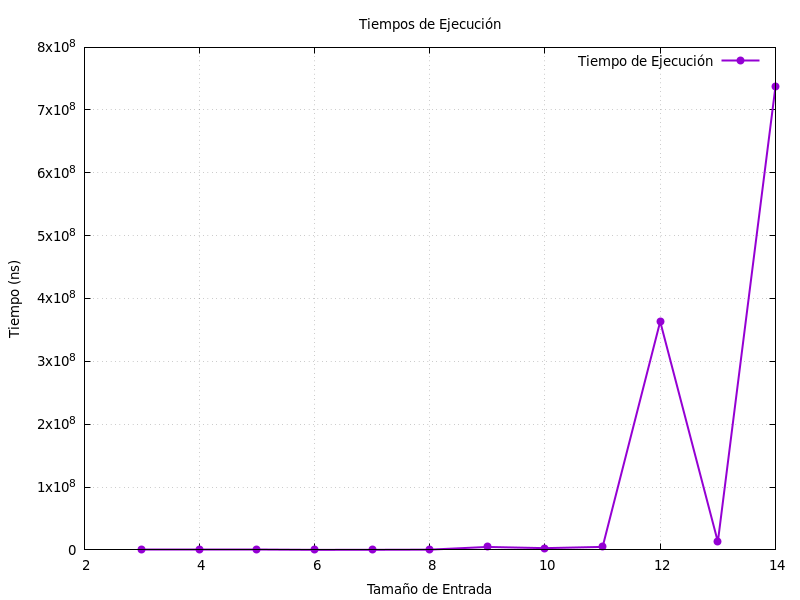
\includegraphics[width=1\linewidth]{assets/Img/Cota_1_BB/grafico_tiempos.png}
            \caption{Cota 1}
            \label{fig:Cota 1}
      \end{minipage}%
      \begin{minipage}{.48\textwidth}
            \centering
            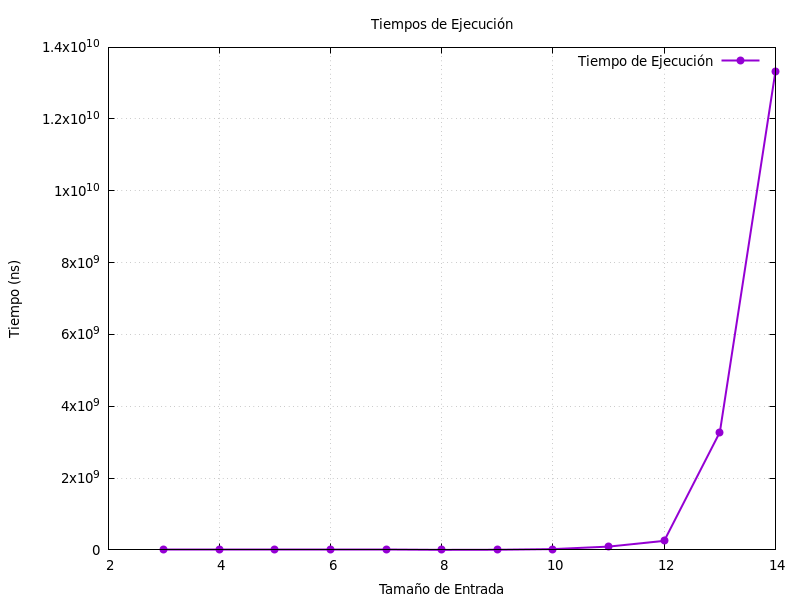
\includegraphics[width=1\linewidth]{assets/Img/Cota_2_BB/grafico_tiempos.png}
            \caption{Cota 2}
            \label{fig:Cota 2}
      \end{minipage}
\end{figure}
\newpage

\section{Justificación}

Para demostrar que el algoritmo Branch and Bound que hemos creado nos proporciona una solución óptima, realizaremos una
demostración por reducción al absurdo. Proposiciones:
\begin{enumerate}
      \item Llamaremos N al conjunto de todos los nodos pertenecientes al último nivel
      \item Llamaremo T al conjunto de todos los nodos pertenecientes a niveles superiores que están podados.
      \item Llamaremos $N_A$ al nodo que nos devuelve nuestro algoritmo
      \item Llamaremos $k_i$ al camino correspondiente de $N_i$
      \item Llamaremos $c_i$ a la cota inferior local correspondiente de $N_i$
      \item Llamaremos C a la cota global
      \item Supondremos que una solución es la óptima cuando en el último nivel del árbol de estado exista
      un camino tal que $k_i \leq k_j \ \ \ \forall N_j \in N$ y que cumpla que $k_i \leq c_{ln}  \ \ \ c_{ln} \in T $ donde 
      n indica el nivel de su ultimo desarrollo, es decir, su rama esta podada 
\end{enumerate}

Procedemos ahora a realizar la reduccioón al absurdo.
Empezamos suponiendo que la solución devuelta no es la óptima, entonces pueden ocurrir dos cosas:
\begin{enumerate}
    \item Existe un nodo en el último nivel al que llamaremos $N_j$ tal que $ N_j \in N$ que cumple que
     $k_j < k_A  \ \ $  entonces  $ N_j$  sería una mejor solución que $N_A$. De hecho, en prticular, se cumpliría que
     $ \exists N_j \in N \text{tal que } k_l \leq k_i  \ \ \forall N_i \in N $. Por tanto, nuestro algoritmo hubiera 
     devuelto $N_j$ en vez de $N_A$ y llegamos a una contradicción
    \item Existiría un nodo $N_{jm} \in T \text{tal que } c_{jm} < K_A = C$ del nivel m, donde la rama estaría podada
    por lo que llegamos a una contradicción, ya que debería seguir desarrollandose al ser menor que la cota global. 
\end{enumerate}

Como podemos ver en ambos casos llegamos a contracción que es lo que buscábamos

\newpage

\section{Gráficas}
Finalmente, mostraremos varias ejecuciones del algoritmo del viajante mediante el Branch and Bound. Mostraremos gráficas realizadas con ambas
cotas aunque eso no se ve reflejado en el resultado final sino más bien en el tiempo de ejecución como hemos mostrado previamente.

\begin{figure}[H]
      \centering
      \begin{minipage}{.48\textwidth}
            \centering
            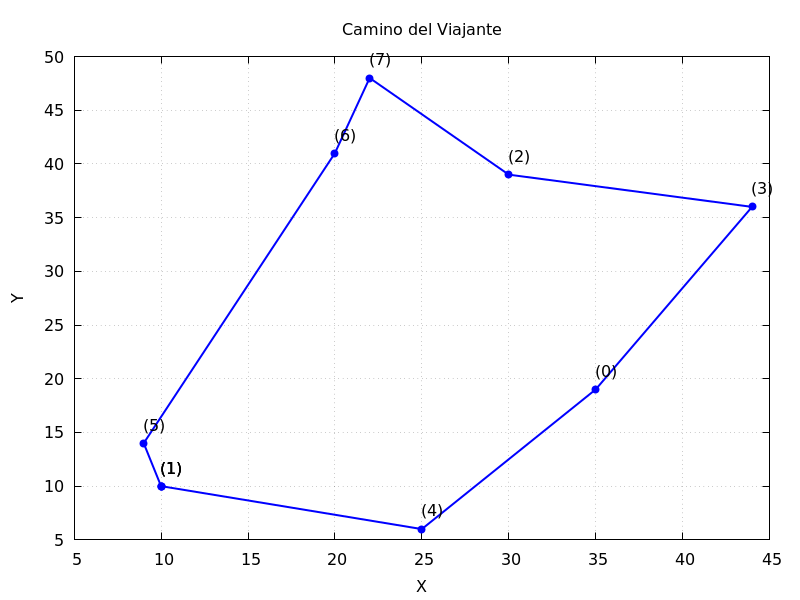
\includegraphics[width=1\linewidth]{assets/Img/Cota_1_BB/grafico_8_1.png}
            \caption{Cota 1, 8 puntos}
            \label{fig:Cota 1}
      \end{minipage}%
      \begin{minipage}{.48\textwidth}
            \centering
            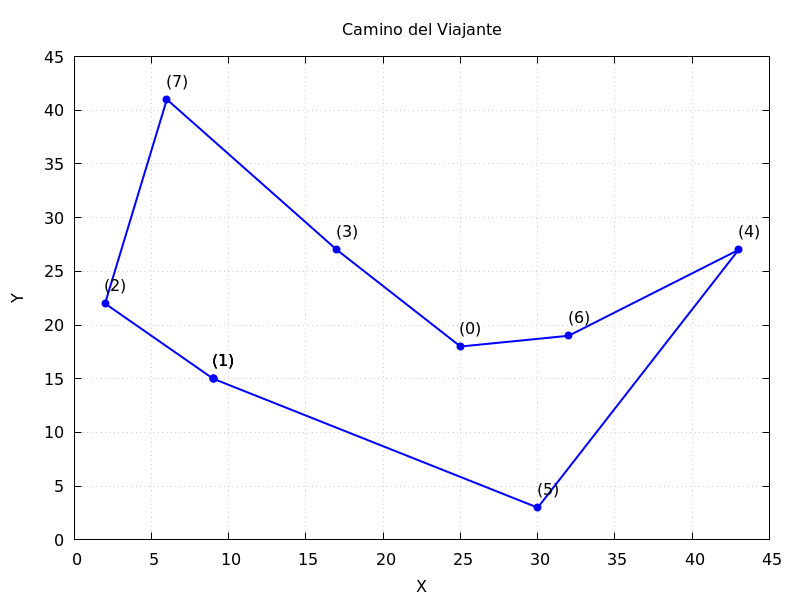
\includegraphics[width=1\linewidth]{assets/Img/Cota_2_BB/grafico_8_1.png}
            \caption{Cota 2, 8 puntos}
            \label{fig:Cota 2}
      \end{minipage}
\end{figure}

\begin{figure}[H]
      \centering
      \begin{minipage}{.48\textwidth}
            \centering
            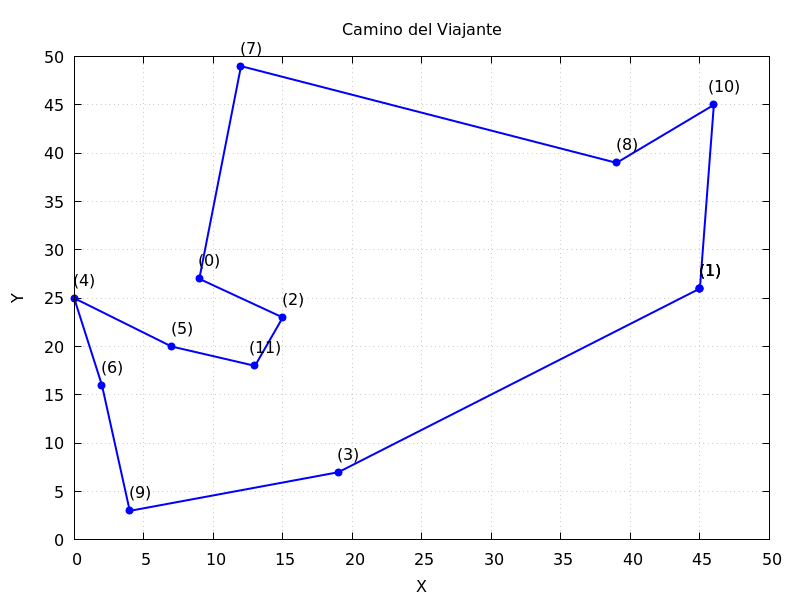
\includegraphics[width=1\linewidth]{assets/Img/Cota_1_BB/grafico_12_1.png}
            \caption{Cota 1, 12 puntos}
            \label{fig:Cota 1}
      \end{minipage}%
      \begin{minipage}{.48\textwidth}
            \centering
            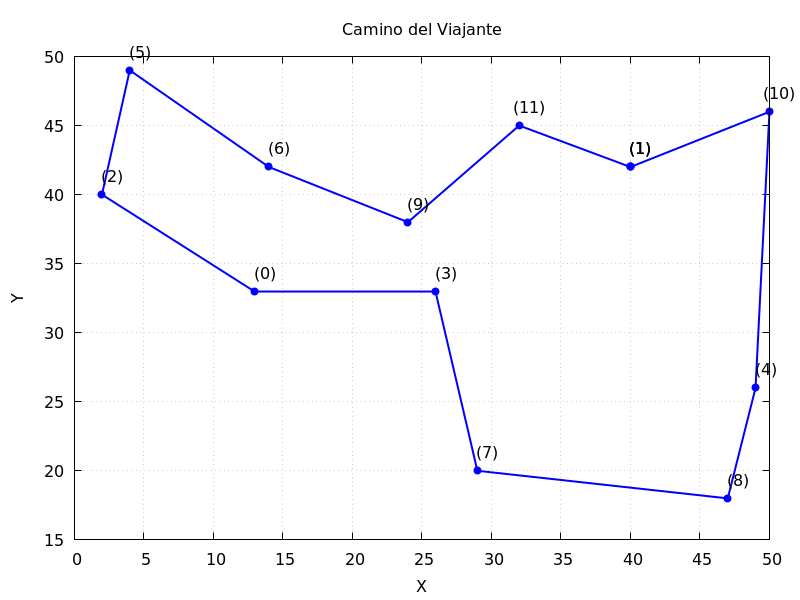
\includegraphics[width=1\linewidth]{assets/Img/Cota_2_BB/grafico_12_1.png}
            \caption{Cota 2, 12 puntos}
            \label{fig:Cota 2}
      \end{minipage}
\end{figure}

A simple vista podemos apreciar que verdaderamenta obtenemos resultados correctos independietmente de la 
cota utilizada, sin embargo, sigue siendo un factor a tener en cuenta devido a la diferencia de tiempo a la 
hora de la ejecución.
\end{document}
